\appendix
\chapter{Appendices}
\section{Algorithm Execution Example}
\subsection{Sparse Offset Computation Algorithm}
\label{ch:spaoffexec}

	This appendix presents an execution of the algorithm \ref{alg:sparseOffsets} presented in section \ref{sssec:sparseOff}.
	
	Let's start with an 4-order tensor $myTensor$  with a shape equal to $[2, 4, 4, 5]$ on which we are calling the following operation:
	
	\begin{lstlisting}[style=nonumbers]
	myTensor.get(NDArrayIndex.all(),
	NDArrayIndex.point(0),
	NDArrayIndex.point(3),
	NDArrayIndex.all());
	\end{lstlisting}
	
	Assuming that $myTensor$ is a view of a 5-order tensor and has a the following parameters:
	
	\begin{lstlisting}[style=nonumbers]		
	sparseOffsets = [1, 1, 0, 0, 0]
	flags = [1, 0, 0, 0, 0]
	\end{lstlisting}
	
	Assuming we name the dimension as [book, page, row, column], we are taking each column of the last row of the first pages of each book.
	
	The indexes resolution returns the following parameters:
	
	\begin{lstlisting}[style=nonumbers]
	offsets = [0, 0]
	shape =  [2, 5]
	offset = 15
	\end{lstlisting}
	
	First step is to iterate over the dimension:\\
	\textbf{Iteration: i=0}\\
	Number of element in one book: $numElement = 4\times 4\times 5 = 60$ \\
	Book offset = $\lfloor offset/numElement\rfloor =  \lfloor 15/60\rfloor = 0$\\  
	Then we update the offset: $offset = offset - 0 * 60$\\
	\textbf{Iteration: i=1}\\
	Number of element in one page = $numElement = 4\times 5 = 20$ \\
	Page offset = $\lfloor offset/numElement\rfloor =  \lfloor 15/20\rfloor = 0$ \\ 
	Then we update the offset: $offset = 15 - 0 * 20$\\
	\textbf{Iteration: i=2}\\
	Number of element in one row = $numElement = 5$\\
	Page offset = $\lfloor offset/numElement\rfloor =  \lfloor 15/5\rfloor = 3$ \\ 
	Then we update the offset: $offset = 15 - 3 * 5 = 0$\\
	
	Finally we reach the last dimension:\\
	Column offset = $offset \mod numElement = 0 \mod 5 = 0$
	
	We get an temporary offsets array equal to $ newOffsets = [0, 0, 3, 0]$. Now we need to merge with the existing offsets of $myTensor$.
	
	Its first dimension (shelf) is fixed, so we copy its sparse offset :\\ $finalOffest[0] = myTensor.sparseOffset[0] = 1$\\
	Its second dimension (book) is active and there is already an non-zero offset. The offset is equal to\\ $finalOffset[1] = newOffset[0] + myTensor.sparseOffset[1] = 0 + 1 = 1$\\
	Its third dimension (page)is active. The offset is equal to\\ $finalOffset[2] = newOffset[1] + myTensor.sparseOffset[2] = 0 + 0 = 0$\\
	Its fourth dimension (row) is active. The offset is equal to\\ $finalOffset[3] = newOffset[2] + myTensor.sparseOffset[3] = 3 + 0 = 0$\\
	Its fifth dimension (column) is active. The offset is equal to\\ $finalOffset[4] = newOffset[3] + myTensor.sparseOffset[4] = 0 + 0 = 0$\\
	
	We finally get the final sparseOffset : $[1, 1, 0, 3, 0]$
	
	
\subsection{Indexes Translation Algorithm}
\label{ssec:idxtrans}
	
	We present an execution of the algorithm \ref{alg:translation} presented in section \ref{ssec:translation}
	
	Let's start with a 3-order tensor $myTensor$ which is a view with the following parameters:
		
	\begin{lstlisting}[style=nonumbers]	
		shape = [1, 2, 2]	
		flags = [1, 0, 0]
		hiddenDimension = [0]
		sparseOffsets = [0, 1, 1]
	\end{lstlisting}
	
	
	\begin{figure}[!h]
		\centering
		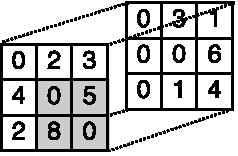
\includegraphics[width=1.5in]{images/apptensors.pdf}
		\caption{A $2\times 3\times 3$ tensor with a view in grey}
		\label{fig:appTensor}
	\end{figure}
	
	The figure \ref{fig:appTensor} shows the tensor $myTensor$ in grey: it's a sup-part of a $2\times 3\times 3$ from which we performed the following operation:
	
	\begin{lstlisting}[style=nonumbers]	
		myTensor = original.get(NDArrayIndex.newAxis(),
			NDArrayIndex.point(0),
			NDArrayIndex.interval(1, 3),
			NDArrayIndex.interval(1, 3));
	\end{lstlisting}

	Let's translate the coordinates of the value 5. In $myTensor$ they are equal to $[0, 0, 1]$ while in $original$ tensors they are equal to $[0, 1, 2]$.
	
	First we start the initilizing phase: the \textit{result} array has a length of three (equal to the dimensionality of $original$). \textit{idxPhy} is used to keep track of the position in the result array we are computing. \textit{hidden} counts the number of hidden dimension we have encountered in the view.
	
	Then we can start with the iterations: we iterate over all the dimensions of the view (idxVir keeps track of the position of the dimension).
	
	\textbf{Iteration: idxVir=0}\\
	The first condition is satisfied since $hidden=0$ is smaller than the number of hidden dimension of $myTensor$ and its hidden dimension is actually the first 0. In this case this coordinate do not appear in the result, we can skip it and increment $hidden$ to 1
	
	\textbf{Teration: idxVir=1}\\
	The first condition is not satisfied: we have already encountered all the hidden dimensions of $myTensor$.
	
	Then we start iterating as long as the dimension is fixed:
	\begin{enumerate}
		\item  We have $idxPhy=0$, according to the \textit{flags} of the original array, $flags[0] = 1$ which means this dimension of the original array is fixed. We can add the $sparseOffset[0] = 0$ to the result.
		
		We have $result = [0, \O, \O]$ and $idxPhy=1$
		
		\item The second dimension is not fixed ($flags[idxPhy] = 0$). We stop iterating.
	\end{enumerate}
	
	The second dimension is not fixed ($flags[idxPhy] = 0$).  We add $sparseOffsets[idxPhx] + viewIdx[idxVir] = 1 + 0 =  1$ into the result.
	
	We have $result = [0, 1, \O]$, $idxPhy=2$ and $idxVir=2$
	
	\textbf{Iteration: idxVir=2}\\
	This dimension is neither hidden nor fixed. We add $sparseOffsets[idxPhx] + viewIdx[idxVir] = 1 + 1 =  2$ into the result.
	
	We finally get the output: $result = [0, 1, 2]$
	
\section{Code Snippets}
\label{ch:codesnip}
\subsection{Extract a sub-array of a CSR matrix}

\begin{lstlisting}[caption=Extract a sub-array of a CSR matrix\label{lst:getcsc},language=Java]
	public INDArray subArray(ShapeOffsetResolution resolution) {
		
		long[] offsets = resolution.getOffsets();
		int[] shape = LongUtils.toInts(resolution.getShapes());
		
		
		List<Integer> accuColumns = new ArrayList<>();
		List<Integer> accuPointerB = new ArrayList<>();
		List<Integer> accuPointerE = new ArrayList<>();
		
		if (shape.length == 2) {
		
			if (resolution.getOffset() != 0) {
				offsets[0] = (int) resolution.getOffset() / shape()[1];
				offsets[1] = (int) resolution.getOffset() % shape()[1];
			}
			long firstRow = offsets[0];
			long lastRow = firstRow + shape[0];
			long firstElement = offsets[1];
			long lastElement = firstElement + shape[1];
			
			int count = 0;
			int i = 0;
			for (int rowIdx = 0; rowIdx < lastRow; rowIdx++) {	
				
				boolean isFirstInRow = true;
				for (int idx = pointerB.getInt(rowIdx); idx < pointerE.getInt(rowIdx); idx++) {
				
					int colIdx = columnsPointers.getInt(count);
					
					// add the element in the subarray it it belongs to the view
					if (colIdx >= firstElement && colIdx < lastElement && rowIdx >= firstRow && rowIdx < lastRow) {
						
						// add the new column pointer for this element
						accuColumns.add((int) (colIdx - firstElement));
						
						if (isFirstInRow) {
							// Add the index of the first element of the row in the pointer array
							accuPointerB.add(idx);
							accuPointerE.add(idx + 1);
							isFirstInRow = false;
						} else {
							// update the last element pointer array
							accuPointerE.set((int) (rowIdx - firstRow), idx + 1);
						}
					}			
					count++;
				}
				
				// If the row doesn't contain any element and is included in the selected rows
				if (isFirstInRow && rowIdx >= firstRow && rowIdx < lastRow) {
					int lastIdx = i == 0 ? 0 : accuPointerE.get(i - 1);
					accuPointerB.add(lastIdx);
					accuPointerE.add(lastIdx);
				}
				if (rowIdx >= firstRow && rowIdx <= lastRow) {
					i++;
				}
			}
			
			int[] newColumns = Ints.toArray(accuColumns);
			int[] newPointerB = Ints.toArray(accuPointerB);
			int[] newPointerE = Ints.toArray(accuPointerE);
			
			INDArray subarray = Nd4j.createSparseCSR(values, newColumns, newPointerB, newPointerE, shape);
			
			return subarray;
		
		} else {
			throw new UnsupportedOperationException();
		}
	}
		\end{lstlisting}
		
	\subsection{Put a Value into a CSR matrix}
		\begin{lstlisting}[caption=Put a new value into a CSR array\label{lst:putcsc},language=Java]
		public INDArray putScalar(int row, int col, double value) {
		
			int idx = pointerB.getInt(row);
			int idxNextRow = pointerE.getInt(row);
			
			while (columnsPointers.getInt(idx) < col && columnsPointers.getInt(idx) < idxNextRow) {
				idx++;
			}
			if (columnsPointers.getInt(idx) == col) {
				values.put(idx, value);
			} else {
				//Add a new entry in both buffers at a given position
				values = addAtPosition(values, length, idx, value);
				columnsPointers = addAtPosition(columnsPointers, length, idx, col);
				length++;
				
				// shift the indices of the next rows
				pointerE.put(row, pointerE.getInt(row) + 1);
				for (int i = row + 1; i < rows; i++) {
					pointerB.put(i, pointerB.getInt(i) + 1);
					pointerE.put(i, pointerE.getInt(i) + 1);
				}
			}
			return this;
		}
		\end{lstlisting}
		
		\subsection{Add a value into a buffer}
		\begin{lstlisting}[caption=Add a value into a buffer\label{lst:addBuff},language=Java]
		private DataBuffer addAtPosition(DataBuffer buf, long dataSize, int pos, double value) {
		
			DataBuffer buffer = (buf.length() == dataSize) ? reallocate(buf) : buf;
			double[] tail = buffer.getDoublesAt(pos, (int) dataSize - pos);
			buffer.put(pos, value);
			
			// we have to shift right the tail
			for (int i = 0; i < tail.length; i++) {
				buffer.put(i + pos + 1, tail[i]);
			}
			return buffer;
		}
		
		\end{lstlisting}
